\documentclass[11pt]{article}
\usepackage[utf8]{inputenc}
\usepackage{hyperref, amsmath, amssymb, amsthm, graphicx, fancyvrb, enumitem, titlesec, setspace, float, fancyvrb, minted}
\usepackage[dvipsnames]{xcolor}
\usepackage[top=1in, bottom=1in, left=1.25in, right=1.25in]{geometry}

\titleformat{\section}{\normalfont\bfseries}{}{0em}{}
\titlespacing*{\section}{0pt}{1.5ex plus .2ex minus .2ex}{0.8ex plus .1ex}
\begin{document}
\noindent Andre Winkel \hfill \today \\
\rule{\textwidth}{0.4pt}

\begin{center} \large {\textbf{Lab 1}} \\[0em] {EE141, Digital Signal Processing, Fall 2025} \end{center}

\section{Problem 1: Converting functions into zero-pole-gain form}
In this problem, we are given a series of functions in transfer function form 
to convert into zero-pole-gain form. We can do so by using the \texttt{matlab} function 
\texttt{roots(coefficients)} to find the zeros and poles of the functions.
\begin{enumerate}[label=\textbf{\alph*)}, leftmargin=2.6em]
    \item Given the transfer function
    \begin{equation} \notag
        H(z) = \frac{2+16z^{-1}+34z^{-2}+20z^{-3}}{1-10z^{-1}+35z^{-2}-50z^{-3}+24z^{-4}}
    \end{equation}
    we can find the zeros and poles by finding the roots of the numerator and denominator, respectively.
    Finding them in MATLAB and plugging them into our standard zero-pole-gain form, we get
    \begin{equation} \notag
        H(z) = 2\frac{z(z+1)(z+2)(z+5)}{(z-1)(z-2)(z-3)(z-4)}.
    \end{equation}

    \item Given the transfer function
    \begin{equation} \notag
        H(z) = \frac{10-21z^{-1}+14z^{-2}-3z^{-3}}{3-3z^{-1}-6z^{-2}}
    \end{equation}
    we do the same process as above to find the zeros and poles. Finding them in MATLAB gives us 
    \begin{equation} \notag
        H(z) = \frac{10}{3}\frac{(z-0.5)(z-0.6)(z-1)}{z(z+1)(z-2)}.
    \end{equation}

    \item And again, given the transfer function
    \begin{equation} \notag
        H(z) = \frac{1-z^{-4}}{1-z^{-8}}
    \end{equation}
    we find our poles, zeros, and gain which reduce to
    \begin{equation} \notag
        H(z) = \frac{z^{4}}
        {(z+\frac{\sqrt2}{2}-\frac{\sqrt2}{2}j)(z+\frac{\sqrt2}{2}+\frac{\sqrt2}{2}j)(z-\frac{\sqrt2}{2}-\frac{\sqrt2}{2}j)(z-\frac{\sqrt2}{2}+\frac{\sqrt2}{2}j)}.
    \end{equation}
\end{enumerate}


\section{Problem 2: Converting functions into transfer function form}
In this problem, we are given a series of functions in pole-zero-gain form
to convert into transfer function form. We can do so by using the \texttt{matlab} function
\texttt{poly(roots)} to find the polynomial that correlates to the provided roots.
\begin{enumerate}[label=\textbf{\alph*)}, leftmargin=2.6em]
    \item Given the pole-zero-gain function
    \begin{equation} \notag
        H(z) = 8 \frac{(z-5)(z+3)(z-1)}{(z-6)(z+11)(z+2)}
    \end{equation}
    we can find the polynomials corresponding to the poles and zeros in MATLAB. We 
    can plug the polynomials and gain into our standard transfer function form, wherein we observe
    our transfer function as
    \begin{equation} \notag
        H(z) = 8\frac{z^3-3z^2-13z+15}{z^3-7z^2-56z+132}.
    \end{equation}
    In standard form, this is equivalent to
    \begin{equation} \notag
        H(z) = \frac{8-24z^{-1}-104z^{-2}+120z^{-3}}{1+7z^{-1}-56z^{-2}-132z^{-3}}.
    \end{equation}

    \item Given the pole-zero-gain function
    \begin{equation} \notag
        H(z) = 2\frac{(z-2)(z-2-j)(z-2+j)}{(z-3)(z+2)(z+j)(z-j)}
    \end{equation}
    we follow the same steps as before to find the transfer function
    \begin{equation} \notag
        H(z) = \frac{2-12z^{-1}+26z^{-2}-20z^{-3}}{1-z^{-1}-5z^{-2}-1z^{-3}-6z^{-4}}.
    \end{equation}

    \item Given the pole-zero-gain function
    \begin{equation} \notag
        H(z) = -3\frac{(z+1)(z-1)(z+j)(z-j)}{z(z-2)}
    \end{equation}
    we follow the same steps as before to find the transfer function
    \begin{equation} \notag
        H(z) = \frac{-3z^2+3z^{-2}}{1-2z^{-1}}.
    \end{equation}
\end{enumerate}


\section{Problem 3: Finding partial fraction expansions}
In this problem, we are given a series of functions to convert into partial fraction form. 
We can do so by using the \texttt{matlab} function \texttt{[r,p,k]=residue(b,a)} 
to find the partial fraction expansion of the given functions.
\begin{enumerate}[label=\textbf{\alph*)}, leftmargin=2.6em]
    \item Given the function
    \begin{equation} \notag
        H(z) = 2\frac{(z+1)(z-1)}{z(z-4)}
    \end{equation}
    we can call the MATLAB function to find that our corresponding values allow us to 
    directly plug in values to observe the standard partial fraction expansion form as
    \begin{equation} \notag
        H(z) = \frac{7.5}{z-4} + \frac{0.5}{z} + 2.
    \end{equation}

    \item Doing the same for the function
    \begin{equation} \notag
        H(z) = \frac{z^3+1}{z^2+1}
    \end{equation}
    we observe
    \begin{equation} \notag
        H(z) = \frac{-0.5-0.5j}{z-j} + \frac{-0.5+0.5j}{z+j} + z.
    \end{equation}
\end{enumerate}


\section{Problem 4: Plotting the pole-zero diagrams}
In this problem, we will plot the pole-zero diagrams using our values obtained in problem 1.
We will use the \texttt{zplane(zeros, poles)} function to plot the pole-zero diagrams.
\begin{enumerate}[label=\textbf{\alph*)}, leftmargin=2.6em]
    \item For the first transfer function, we observe the following plot: 
    \begin{figure} [H]
        \centering
        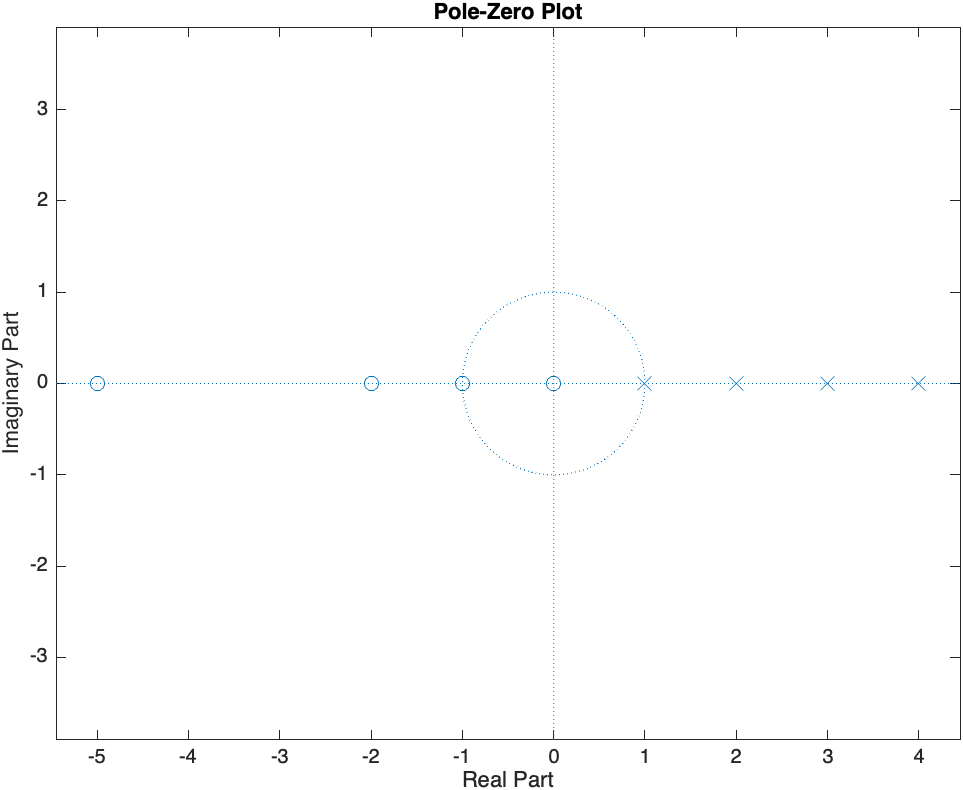
\includegraphics[width=0.5\linewidth]{fig1.png}
    \end{figure}

    \item Again, for the second transfer function, we observe the following:
    \begin{figure} [H]
        \centering
        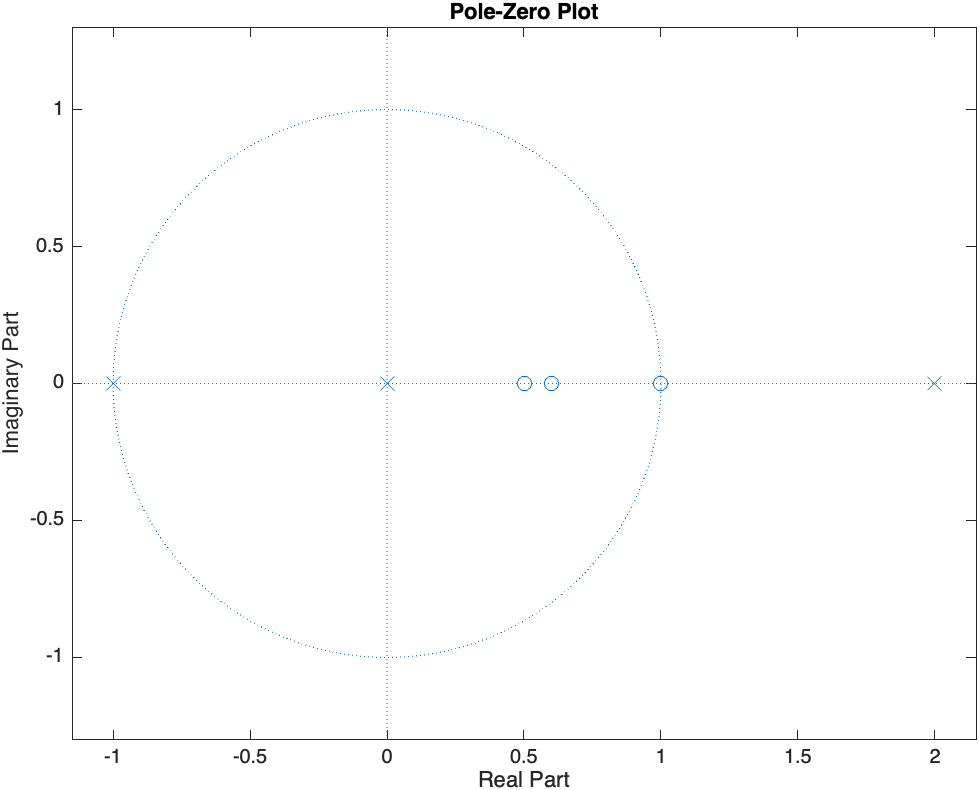
\includegraphics[width=0.5\linewidth]{fig2.png}
    \end{figure}

    \item And finally:
    \begin{figure} [H]
        \centering
        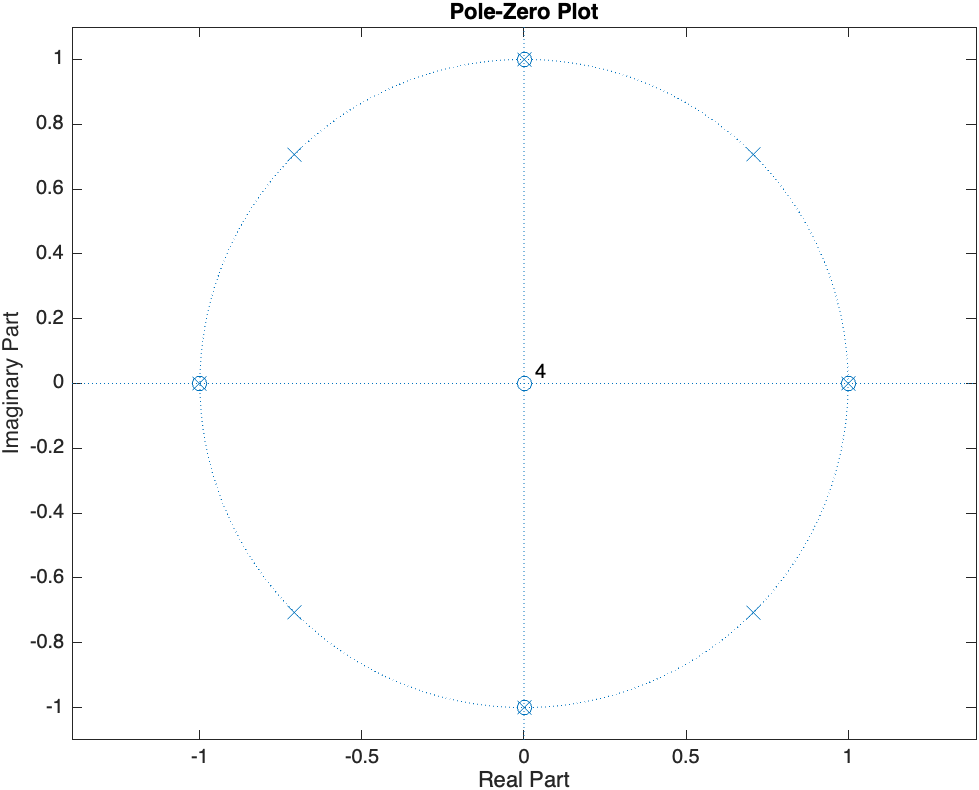
\includegraphics[width=0.5\linewidth]{fig3.png}
    \end{figure}
\end{enumerate}

\end{document}